\section{Conclusiones}

\subsection{Bordes}
En caso de una imagen con cambios grandes en zonas pequeñas, todos los algoritmos tienden a fallar en esas zonas.
Esto se debe a que todos los algoritmos dependen fuertemente de los pixeles próximos cercanos, los cuales poseen valores muy distintos al valor a calcular. Esto es denominado borde.

\subsection{Comparación de calidad}
En esta sección compararemos solo los verdes de las imágenes y veremos los resultados utilizando PSNR. Recordemos que este término, calcula nivel de ruido en una señal.

\begin{figure}[h]
       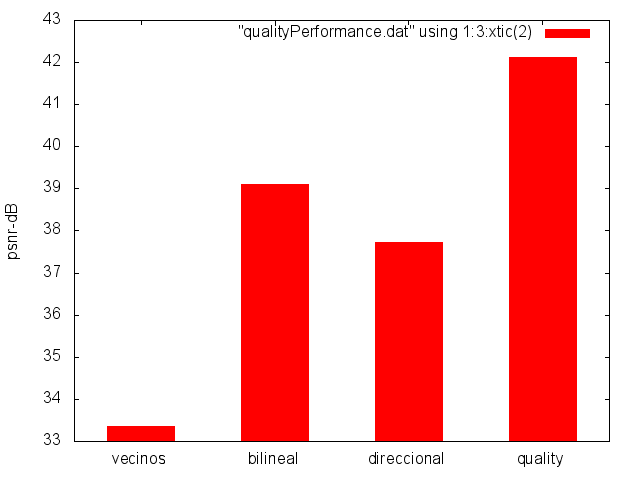
\includegraphics[width=1\textwidth]{imagenes/quality_performance.png}
\end{figure}

Como era esperado, el vecinos es el que peor hizo, y quality fue el mejor. Sin embargo notemos que Spline si bien tendría que tener un valor mayor que bilineal ya que subjetivamente notamos mejora entre ellos, no lo tiene, es decir, el nivel de ruido es mayor en el direccional. Esto tiene sentido en la medida que el algoritmo direccional utiliza toda la fila y toda la columna para calcular el valor de las coordenadas $b_j$, $c_j$ y $d_j$ por lo que está sujeto a valores distintos al valor final, a diferencia de Bilineal que está sujeto a sus vecinos directos que es mucho más probable que tengan un valor más próximo.